\section{Interacting with Flags API} \label{section: api}

The method \texttt{getCountryAndQuoteFromServer} contains everything related to the flags API. This method is run when you are playing JavaCraft and the command \texttt{getflag} is typed. The method initially did not contain and json or a valid url, which has been changed. The updated part of the code can be found below. Note that only the modified parts of the code are included in the method: the unmodified parts are replaced with ellipses surrounded by brackets: 

\begin{lstlisting}
    public static void getCountryAndQuoteFromServer() {
    try {
      String link = "https://flag.ashish.nl/get_flag";
      URL url = new URL(link);
      [...]
      String payload = "{\n" +
         "    \"group_number\": \"11\",\n" +
         "    \"group_name\": \"group11\",\n" +
         "    \"difficulty_level\": \"hard\"\n" +
         "}";
      [...]
    }
  }
\end{lstlisting}

The flags API and documentation can be found at \url{https://flag.ashish.nl/}. The POST \/get\_flag method requires json that has 3 parameters: \texttt{group\_number}, \texttt{group\_name} and \texttt{difficulty\_level}. When a successful call has been made, the method \texttt{getCountryAndQuoteFromServer} will print a country's name and a quote. In the case of our group \texttt{group11}, the chosen difficulty level was \texttt{hard} and the flag we got is the flag of Bangladesh. \\

The flag of Bangladesh is a dark green flag with a red circle. The flag is constructed as follows:

\begin{center}
  {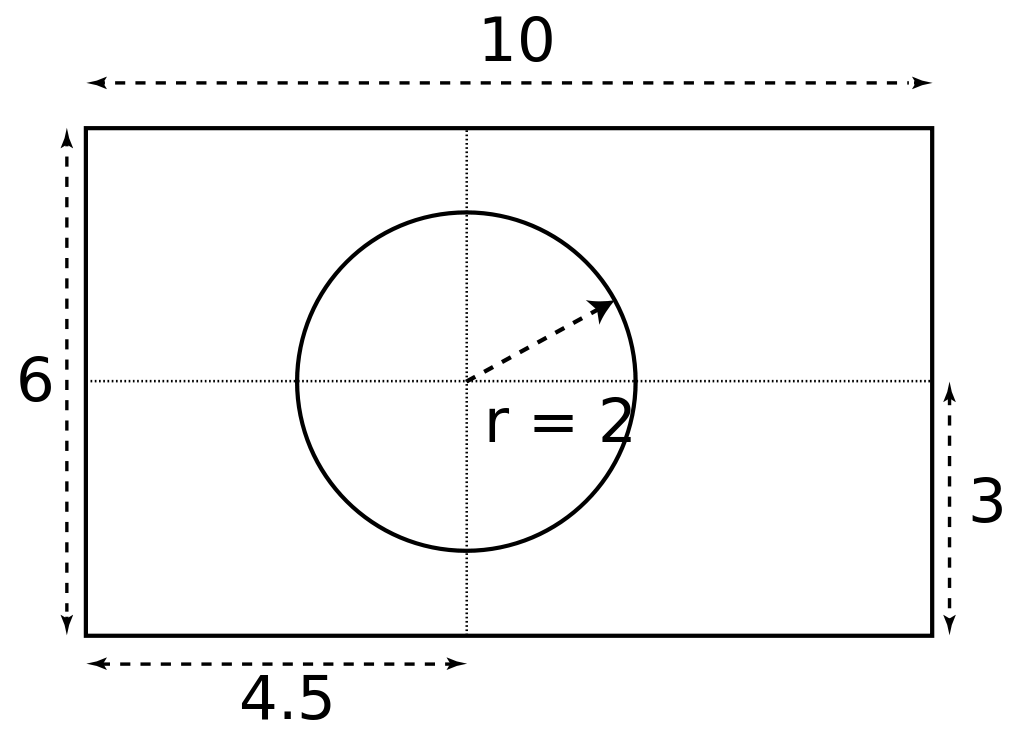
\includegraphics[height=80px]{../bangladesh-construct.png}}
\end{center}

Based on a given width and height, we can determine the center of the circle as well as the radius. \\
Let \(x\) and \(y\) be the width and height of the world respectively. Let \(x_r\) and \(y_r\) be the x and y coordinate of the circle. Let \(r\) be the radius of the circle. Using the ratios of the flag we can conclude that \(x_r = x \cdot \frac{4.5}{10}\) and \(y_r = y \cdot \frac{1}{2}\) and \(r = \frac{2}{10}x = \frac{2}{6}y\). The formula of the circle goes as follows:
\begin{center}
  \((x - x_r)^2 + (y - y_r)^2 = r^2\)
\end{center}
We now loop through every coordinate of the flag. If the condition \((x - x_r)^2 + (y - y_r)^2 \le r^2\) is true it means that at that given x and y coordinate the coordinates are inside of the circle. We then render the square to be red. If the condition is not met then the square is green.
\begin{lstlisting}
  private static void generateEmptyWorld() {
    world = new int[NEW_WORLD_WIDTH][NEW_WORLD_HEIGHT];
    int xCircleCenter = (NEW_WORLD_WIDTH * 9/20);
    int yCircleCenter = NEW_WORLD_HEIGHT / 2;
    int r = (NEW_WORLD_WIDTH / 10 * 2); 
     for (int y = 0; y < NEW_WORLD_HEIGHT; y++) {
      for (int x = 0; x < NEW_WORLD_WIDTH; x++) {
        if ((x-xCircleCenter)*(x-xCircleCenter)+(y-yCircleCenter)*(y-yCircleCenter) <= r*r) {
          world[x][y] = REDBLOCK;
        } else { world[x][y] = GREENBLOCK; }
      }
    }
  }
\end{lstlisting}